% Created 2020-10-07 Wed 11:32
% Intended LaTeX compiler: lualatex
\documentclass[11pt]{article}
\usepackage{graphicx}
\usepackage{grffile}
\usepackage{longtable}
\usepackage{wrapfig}
\usepackage{rotating}
\usepackage[normalem]{ulem}
\usepackage{amsmath}
\usepackage{textcomp}
\usepackage{amssymb}
\usepackage{capt-of}
\usepackage{hyperref}
\usepackage{tabularx}
\usepackage{etoolbox}
\makeatletter
\def\dontdofcolorbox{\renewcommand\fcolorbox[4][]{##4}}
\AtBeginEnvironment{minted}{\dontdofcolorbox}
\makeatother
\usepackage[newfloat]{minted}
\usepackage{amsthm}
\theoremstyle{definition}
\newtheorem{definition}{Definition}[section]
\usepackage{unicode-math}
\usepackage{unicode}
\author{Mark Armstrong}
\date{Fall 2020}
\title{An untyped λ-calculus, \emph{UL}\\\medskip
\large Principles of Programming Languages}
\hypersetup{
   pdfauthor={Mark Armstrong},
   pdftitle={An untyped λ-calculus, \emph{UL}},
   pdfkeywords={},
   pdfsubject={Our first constructed language; a lambda calculus with no type checking (enforcement).},
   pdfcreator={Emacs 27.0.90 (Org mode 9.4)},
   pdflang={English},
   colorlinks,
   linkcolor=blue,
   citecolor=blue,
   urlcolor=blue
   }
\begin{document}

\maketitle

\section{Preamble}
\label{sec:org3a5490e}
\subsection{{\bfseries\sffamily TODO} Notable references}
\label{sec:orgd0b2226}
\begin{itemize}
\item Benjamin Pierce,
“\href{https://ebookcentral.proquest.com/lib/mcmu/detail.action?docID=3338823}{Types and Programming Languages}”
\begin{itemize}
\item Chapter 5, The Untyped Lambda-Calculus
\end{itemize}
\end{itemize}

\subsection{{\bfseries\sffamily TODO} Table of contents}
\label{sec:org33e79a6}
\begin{scriptsize}
\begin{itemize}
\item \hyperref[sec:org3a5490e]{Preamble}
\end{itemize}
\end{scriptsize}

\section{Introduction}
\label{sec:orga8e2892}
In this section we construct our first simple programming language,
an untyped λ-calculus (lambda calculus).

More specifically, we construct a λ-calculus
without (static) type checking (enforcement),
but including the natural numbers and booleans.

\subsection{What is the λ-calculus?}
\label{sec:org781e137}
The λ-calculus is, put simply,
a notation for forming and applying functions.
\begin{itemize}
\item Because the function (procedure, method, subroutine) abstraction
gives us a means of representing control flow,
if we have a means of representing data,
the λ-calculus is a Turing-complete model of computation.
\end{itemize}

\subsection{History}
\label{sec:org25a142f}
The (basic) λ-calculus as we know it was famously invented
by Alonzo Church in the 1920s.
\begin{itemize}
\item This was one culmination of a great deal of work by
mathematicians investigating the foundations of mathematics.
\end{itemize}

As mentioned, the λ-calculus is a Turing-complete model of computation.
\begin{itemize}
\item Other models proposed around the same time include
\begin{itemize}
\item the Turing machine itself (due to Alan Turing), and
\item the general recursive functions (due to Stephen Cole Kleene.)
\end{itemize}
\item Hence the “Church” in the “Church-Turing thesis”.
\end{itemize}

The λ-calculus has since seen widespread use in the study and design
of programming languages.
\begin{itemize}
\item It is useful both as a simple programming language, and
\item as a mathematical object about which statements can be proved.
\end{itemize}

\subsection{Descendents of the λ-calculus}
\label{sec:orge9fbe0e}
Pure functional programming languages are clearly descended
from the λ-calculus; the λ-calculus embodies their model of computation.
\begin{itemize}
\item Additionally, it is common to have a “lambda” operator
which allows definition of anonymous functions.
\begin{itemize}
\item This is so even outside of pure functional languages,
\begin{itemize}
\item and it is becoming common
in primarily imperative languages as well!
\end{itemize}
\end{itemize}
\end{itemize}

Imperative languages instead (traditionally) use a model of computation
based on the \emph{Von-Neumann} architecture,
\begin{itemize}
\item which matches our real-world computing devices!
\begin{itemize}
\item Hence imperative languages are naturally lower-level;
one level of abstraction closer to the real computer
that functional languages, which must be translated
to imperative code in order to run.
\end{itemize}
\item This model of computation is a natural extension
of the Turing machine, rather than the λ-calculus
or recursive functions.
\end{itemize}

\section{The basics}
\label{sec:orgc60885c}
In our discussion of abstractions, we mentioned
the abstraction of the function/method/procedure/subroutine.
\begin{itemize}
\item The functional abstraction provides a means
to represent control flow.
\end{itemize}

In its pure version, every term in the λ-calculus
is a function.
\begin{itemize}
\item In order for such a system to be at all useful,
it must of course support higher-order functions;
functions may be applied to functions.
\item Values such as booleans and natural numbers
are \emph{encoded} (represented) by functions.
\end{itemize}

\subsection{Informal definition of terms}
\label{sec:org5fc934d}
The pure untyped λ-calculus has just three sort of terms;
\begin{itemize}
\item variables such as \(x\), \(y\), \(z\),
\item \emph{λ-abstractions}, of the form \(λ x → t\),
\begin{itemize}
\item (it is also common to use \(․\) in place of \(→\);
we prefer \(→\) as it emphasises that these are functions)
\item where \(x\) is a variable and \(t\) is a λ-term, and
\end{itemize}
\item applications of the form \(t u\)
\begin{itemize}
\item where \(t\) and \(u\) are λ-terms.
\end{itemize}
\end{itemize}

\subsection{Informal meaning of terms}
\label{sec:orgb6a7c86}
The meaning of each term is, informally:
\begin{itemize}
\item A λ-abstraction \(λ x → t\) represents a function of one argument,
which, when applied to a term \(u\), substitutes
all free occurrences of \(x\) in \(t\) with \(u\).
\item An application applies the term \(u\) to the function (term) \(t\).
\item A variable on its own (a free variable) has no further meaning.
\begin{itemize}
\item Variables are intended to be \emph{bound}.
\item “Top-level” free variables have no meaning (on their own).
\begin{itemize}
\item Until we construct a new term by λ-abstracting them.
\end{itemize}
\end{itemize}
\end{itemize}

\subsection{Variable binding}
\label{sec:orga002952}
Recall the notion of free and bound variables.
\begin{itemize}
\item A \emph{variable binder} is an operator which operates on
some number of \emph{variables} as well as \emph{terms}.
\begin{itemize}
\item Examples include quantifiers
such as \(∀\_❙\_•\_\), \(∃\_❙\_•\_\) and \(∑\_❙\_•\_\),
and substitution \(\_[\_→\_]\).
\item By convention, the bodies of variable binders extend as far
to the right as possible;
\begin{itemize}
\item so for instance \(∀ x ❙ P x • Q x ∧ R y\) is read
as \((∀ x ❙ P x • (Q x ∧ R y))\).
\end{itemize}
\item But substitution binds tighter than any other operation;
\begin{itemize}
\item so for instance \(x + y [y ≔ z]\) is read as \(x + (y [y ≔ z])\)
\end{itemize}
\end{itemize}
\end{itemize}

\subsection{Free and bound variables}
\label{sec:orga4c82c9}

For simplicity, let us assume here that variable binders
act on a single variable and a single term.
\begin{itemize}
\item Let \(B\_•\_\) range over the set of variable binders in a language.
\item An occurrence of a variable \(x\) in a term \(t\) that is \emph{not} in
a subterm of the form \(B x • u\) is called \emph{free}.
\item In a term \(t\) with a subterm of the form \(B x • u\),
all free occurrences of the variable \(x\) that occur within \(u\)
are \emph{bound} by that instance of the binder \(B\).
\begin{itemize}
\item Note: instances of \(x\) which are bound elsewhere are not bound
by that \(B\).
\end{itemize}
\end{itemize}

\subsection{Open and closed terms; combinators}
\label{sec:org97349ad}

\begin{itemize}
\item A λ-term which contains free variables is called an \emph{open term}.

\item A λ-term with no free variables is called a \emph{closed term}.
\begin{itemize}
\item Such λ-terms are also called \emph{combinators}.
\end{itemize}
\end{itemize}

\subsection{Picturing variable bindings}
\label{sec:orgc241257}
For instance, in the language of predicate logic,
we can view the variables bound like so.
\begin{center}
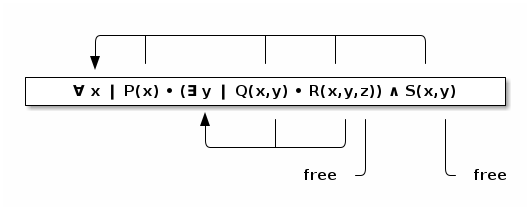
\includegraphics[width=\textwidth]{media/variable-binding.png}
\end{center}

\subsection{Representing functions with multiple arguments}
\label{sec:org2af8b1f}
You may have noticed that our method for constructing function
in the λ-calculus (the λ-abstraction)
only allows us to construct single-argument functions.
\begin{itemize}
\item That is, we do not have terms such as \(λ(x,y) → t\).
\item This may seem restrictive,
\item but it turns out to be sufficient.
And it keeps the language simpler theoretically.
\end{itemize}

\subsection{Currying}
\label{sec:org60dbf92}
Rather than complicating our set of terms by admitting
functions of multiple arguments, we use the technique
of \emph{currying} functions.
\begin{itemize}
\item Consider a function \(f : A × B → C\).
\item We can substitute a new function \(f′ : A → (B → C)\)
for \(f\).
\begin{itemize}
\item (By convention, function arrows associate to the right,
so this is equivalent to \(f : A → B → C\).)
\item So \(f′\) is a function which takes an \(A\) and
\emph{produces a function} of type \(B → C\).
\begin{itemize}
\item We also say that \(f′\) is \emph{partially applied} to a value of \(A\).
\item We usually don't give this new function a name.
\item We can consider this new function as having a \emph{fixed} value
for the \(A\) argument that was provided.
\item (So we must be able to represent higher-order functions
to use Currying.)
\end{itemize}
\end{itemize}
\end{itemize}

\subsection{Examples of λ-terms}
\label{sec:org8a58bb8}
\begin{minted}[breaklines=true]{text}
λ x → x
\end{minted}
is a familiar function; it is the \emph{identity} function.
We will use the name \texttt{id} to refer to this function.

\begin{minted}[breaklines=true]{text}
λ x → λ y → x
\end{minted}
is a function which ignores its second argument,
and just returns the first; this is sometimes called \texttt{const}.

\begin{minted}[breaklines=true]{text}
λ x → λ y → y
\end{minted}
is then a function which ignores its first argument.

\begin{minted}[breaklines=true]{text}
λ f → λ x → f x
\end{minted}
is a function which applies its second argument to its first;
we might call this just \texttt{apply}.

\section{The syntax and semantics of \emph{UL}}
\label{sec:org3e03b0e}
We now discuss the formal semantics of the untyped λ-calculus;
that is, we
\begin{itemize}
\item give a grammar for its syntax, and
\item define operational semantics for the language.
\end{itemize}

\subsection{A grammar for \emph{UL}}
\label{sec:orge19706f}
\begin{minted}[breaklines=true]{text}
⟨term⟩ ∷= var | λ var → ⟨term⟩ | ⟨term⟩ ⟨term⟩
\end{minted}

In the case that we are restricted to ASCII characters,
we will write abstraction as
\begin{minted}[breaklines=true]{text}
“lambda” var . ⟨term⟩
\end{minted}

\subsection{The operational semantics of \emph{UL}}
\label{sec:orgb166ecd}
A term of the form \((λ x → t₁) t₂\) is called a \emph{redex} (β-redex),
meaning \emph{reducible expression}.

The semantics of the λ-calculus is given by a \emph{reduction strategy}
(\emph{β}-reduction strategy);
\begin{itemize}
\item A reduction (β-reduction) transforms a subterm of the form
\begin{itemize}
\item \((λ x → t₁) t₂\) (a redex) to
\item \(t₁[x ≔ t₂]\).
\begin{itemize}
\item (There are various syntactic representations of substitutions;
we prefer to the substitution operation to come after the term
where the substitution is carried out (\(t₁\)), and to use
the “becomes” operator to imply free instance of \(x\) become \(t₂\).
\item Pierce instead uses the form \([x ↦ t₂]t₁\), with the
substitution operation coming before the term,
and using the “maps to” operator instead of “becomes”.
\item You may also see forms such as \([x\backslash t₁]\) or \([t₁/x]\).)
\end{itemize}
\end{itemize}
\end{itemize}

\subsection{Normal forms and values}
\label{sec:org80211d7}

A term which does not involve any redexes is said to be
in \emph{normal form} (β-normal form).
\begin{itemize}
\item Terms in β-normal form which are not variables
are called \emph{values}.
\begin{itemize}
\item In the pure untyped λ-calculus, these only include λ-abstractions.
\item Later, we will add other constant values,
such as \texttt{true}, \texttt{false}, \texttt{0}, etc.
\end{itemize}
\end{itemize}

In the untyped λ-calculus,
\begin{itemize}
\item if a term has a normal form, that normal form is unique.
\begin{itemize}
\item (By the \emph{Church–Rosser} theorem.)
\end{itemize}
\item But not all terms have a normal form!
\end{itemize}

\subsection{Some reduction strategies}
\label{sec:org6836dc9}
Given an arbitrary term, there may be several subterms which are redexes,
\begin{itemize}
\item so we have a choice of what subterm to reduce.
\end{itemize}
A reduction strategy limits our choice of which redex to reduce.

Several strategies have been studied. We discuss just four of them.
\begin{itemize}
\item full β-reduction, normal order,
\item call by name, and call by value.
\end{itemize}
We only give a full formal treatment to call-by-value.

The last two you may know as names of parameter passing methods
from (practical) programming languages.
\begin{itemize}
\item There is a direct correspondance between reduction strategies
and parameter passing methods.
\end{itemize}

\subsection{Some reduction strategies: full β-reduction and normal order}
\label{sec:org48d52c0}
The \emph{full β-reduction} strategy is, essentially, to have no
strategy at all.
\begin{itemize}
\item Under full β-reduction, and redex can be reduced at any point.
\item This strategy gives rise to a reduction \emph{relation},
not a function.
\begin{itemize}
\item Since a given term may reduce to \emph{many} other terms.
\end{itemize}
\end{itemize}

The \emph{normal order} strategy enforces that the
leftmost, outermost redex is always reduced first.
\begin{itemize}
\item This restriction gives rise to a function.
\end{itemize}

\subsection{Some reduction strategies: call by name and call by value}
\label{sec:org4aff36a}
The \emph{call by name} strategy builds on the normal order strategy
\begin{itemize}
\item by mandating that no reductions take place inside abstractions.
\item So “arguments cannot be evaluated before being applied”.
\end{itemize}

The \emph{call by value} strategy also builds on the normal order strategy,
\begin{itemize}
\item by mandating that a redex is reduced only when its right hand side
\begin{itemize}
\item (the “argument”)
\end{itemize}
is a value (in β-normal form and not a variable).
\end{itemize}

\subsection{A formal description of call by value semantics}
\label{sec:org7394385}

Let us use the convention that variable names involving
\begin{itemize}
\item \texttt{t} represent arbitrary λ-terms, whereas variable names involving
\item \texttt{v} represent terms in λ-normal form (values).
\end{itemize}

Then we may give a formal description of call-by-value semantics
using inference rules.
\begin{minted}[breaklines=true]{text}
   t₁ ⟶ t₁′
–––––––––––––––– Appˡ
t₁ t₂ ⟶ t₁′ t₂


   t₂ ⟶ t₂′
–––––––––––––––– Appʳ
v₁ t₂ ⟶ v₁ t₂′

   
–––––––––––––––––––––––– AppAbs
(λ x → t) v ⟶ t[x ≔ v]
\end{minted}
Notice how the use of \texttt{t}'s and \texttt{v}'s mandates that
\begin{itemize}
\item terms on the left reduce first, and
\item applications only take place when the term being applied is a value.
\end{itemize}

\subsection{β-reduction, α-equivalence and η-conversion}
\label{sec:org7891da5}
β-reduction gives us one way to equate terms;
\begin{itemize}
\item two terms “have the same value” if they both reduce to the same
value (irreducible term.)
\item So we call terms that reduce to the same value
β-equivalent.
\begin{itemize}
\item For instance, \((λ x → x) y =_{β} y\).
\end{itemize}
\end{itemize}

Two other notions of equality between λ-terms prove useful.
\begin{itemize}
\item α-equivalence stipulates that two terms which vary
only in the naming of bound variables are equivalent.
\begin{itemize}
\item For instance, \(λ x → x =_{α} λ y → y\).
\item This is a very useful stipulation to help avoid
name clashes!
\end{itemize}
\item η-conversion stipulates that
\begin{itemize}
\item a term of the form \(λ x → f x\) can be reduced to \(f\),
(η-reduction)
and conversely,
\item a term of the form \(f\) can be expanded to \(λ x → f x\)
(η-expansion.)
\end{itemize}
\end{itemize}

\subsection{Strong and weak normalisation}
\label{sec:orga6f4d51}

As we've said, a λ-term is said to be
in \emph{normal form} if it cannot be reduced.
\begin{itemize}
\item We can define this concept of normal form
in any system in which terms reduce;
\begin{itemize}
\item in particular, in all the other models of computation
we will consider.
\end{itemize}
\end{itemize}

A set of terms along with a reduction strategy is then called
\begin{itemize}
\item \emph{strongly normalising} if every reduction sequence is guaranteed
to terminate in a normal form, and
\item \emph{weakly normalising} if for every term, there is at least one
reduction sequence which terminates in a normal form.
\end{itemize}

\subsection{Exercise: a term with no normal form}
\label{sec:orga22fdb5}

One combinator (closed term) of the untyped λ-calculus
is the \emph{ω-combinator}, which is also called the \emph{divergent} combinator.
\begin{minted}[breaklines=true]{text}
omega = (λ x → x x) (λ x → x x)
\end{minted}

This combinator has no normal form; can you prove that?

Hint: what reductions are possible here?
What is the result of that reduction?

\section{λ-encodings}
\label{sec:org3301cfb}
As mentioned previously, in the pure λ-calculus,
every term is a function.
\begin{itemize}
\item There are no basic types of data.
\end{itemize}

So, we must have a way of representing any data as
a function.
\begin{itemize}
\item We call these Church encodings.
\end{itemize}

We will show how to do this for
\begin{itemize}
\item booleans,
\item pairs, and
\item natural numbers,
\end{itemize}
and give some “combinators” which operate on these kinds of data.

\subsection{Church booleans}
\label{sec:org12826ee}

We define the following terms to represent boolean values.
\begin{itemize}
\item \texttt{tru} represents truth, and
\item \texttt{fls} represents false.
\end{itemize}
\begin{minted}[breaklines=true]{text}
tru = λ t → λ f → t
fls = λ t → λ f → f
\end{minted}

These choices are \emph{somewhat} arbitrary.
\begin{itemize}
\item We could choose any two distinct λ-terms.
\item But they are not really arbitrary;
these two terms embody the idea that a boolean value
is a “choice” between two options.
\begin{itemize}
\item \texttt{tru}, when given two arguments, “chooses” the first.
\item \texttt{fls}, when given two arguments, “chooses” the second.
\end{itemize}
\end{itemize}

\subsection{Defining \texttt{if-then-else} using Church booleans}
\label{sec:org372517d}

Since the Church encoded booleans already “perform” a choice,
defining an “if-then-else” construct
using them is quite straightforward.
\begin{minted}[breaklines=true]{text}
test = λ l → λ m → λ n → l m n
\end{minted}
The intention is that
\begin{itemize}
\item the first argument is a Church boolean,
\item the second is the “then” branch, and
\item the third is the “else” branch.
\end{itemize}

Notice that \texttt{test b v w} simply reduces to \texttt{b v w};
\begin{itemize}
\item the boolean \texttt{b} really “does the work”
of choosing between \texttt{v} and \texttt{w}.
\end{itemize}

\subsection{Exercise: is \texttt{test} really if-then-else?}
\label{sec:orgdf9d31e}

Let us briefly pause to consider the semantics of \texttt{test},
\begin{itemize}
\item and see if it matches the behaviour
we expect from an “if-then-else” construct.
\end{itemize}

Consider the example λ-term
\begin{minted}[breaklines=true]{text}
test true (id true) (id false)
\end{minted}

Using call-by-value semantics, we have
\begin{minted}[breaklines=true]{text}
  test true (id true) (id false)
= test true ((λ x → x) (λ x → λ y → x)) ((λ x → x) (λ x → λ y → y))
⟶ test true (λ x → λ y → x) ((λ x → x) (λ x → λ y → y))
⟶ test true (λ x → λ y → x) (λ x → λ y → y)
= test true true false
⟶ …
\end{minted}

Exercise: Considering this portion of the reduction sequence,
what is different about \texttt{test} and the “if-then-else” construct
that you are used to?

\subsection{Pairs}
\label{sec:orga0e777e}

We now give an encoding of pairs
\begin{itemize}
\item (a wrapping of two terms into one),
\item along with pair “deconstructors”.
\end{itemize}
These definitions rely upon the encoding of booleans
we have just given.

\begin{minted}[breaklines=true]{text}
pair = λ f → λ s → λ b → b f s
fst = λ p → p tru
snd = λ p → p fls
\end{minted}

We may check that, for instance, \texttt{fst (pair v w)} will indeed
reduce to \texttt{v}, using call-by-value semantics.
\begin{minted}[breaklines=true]{text}
  fst (pair v w)
= (λ p → p (λ x → λ y → x)) ((λ f → λ s → λ b → b f s) v w)
⟶ (λ p → p (λ x → λ y → x)) ((      λ s → λ b → b v s)   w)
⟶ (λ p → p (λ x → λ y → x)) ((            λ b → b v w))
⟶ (λ b → b v w) (λ x → λ y → x)
→ (λ x → λ y → x) v w
⟶ (λ y → v) w
→ v
\end{minted}

\subsection{Exercise: \texttt{snd}}
\label{sec:org7486301}

As an exercise, you may confirm
that \texttt{snd (pair v w)} reduces to \texttt{w}, using call-by-value semantics.

\subsection{Natural numbers: Church numerals}
\label{sec:org49dbf58}

To represent natural numbers is only slightly more complicated
than booleans and pairs. We give the pattern
\begin{minted}[breaklines=true]{text}
c₀ = λ s → λ z → z
c₁ = λ s → λ z → s z
c₂ = λ s → λ z → s (s z)
…
\end{minted}
That is, each numeral \texttt{n} is represented as the function
which applies its first argument to its second argument \texttt{n} times.

Or more neatly, we define
\begin{minted}[breaklines=true]{text}
zero = λ s → λ z → z
scc = λ n → λ s → λ z → s (n s z)
\end{minted}
so then \texttt{c₀} is \texttt{zero}, \texttt{c₁} can be obtained from \texttt{scc zero} (by reducing it),
\texttt{c₂} can be obtained from \texttt{scc (scc zero)}, etc.

\subsection{Addition and multiplication}
\label{sec:org5bdbb58}

By using the fact that
\begin{itemize}
\item “each numeral \texttt{n} is represented as the function which applies
its first argument to its second argument \texttt{n} times”,
\end{itemize}
we can fairly easily define addition and multiplication.

For addition, \texttt{m + n},
\begin{itemize}
\item we begin with \texttt{n},
\item and apply \texttt{suc} \texttt{m}-many times.
\end{itemize}
\begin{minted}[breaklines=true]{text}
plus = λ m → λ n → λ s → λ z → m s (n s z)
\end{minted}

For multiplication, \texttt{m * n},
\begin{itemize}
\item we begin with \texttt{zero},
\item and apply “\texttt{plus n}” \texttt{m}-many times.
\end{itemize}
\begin{minted}[breaklines=true]{text}
times = λ m → λ n → m (plus n) zero
\end{minted}

\subsection{Testing for zero}
\label{sec:org3091d94}

In order to test if a natural number is zero, we use the same ideas,
\begin{itemize}
\item but now the base case is true,
\item and the function we apply \texttt{m}-many times
is just the constantly false function.
\end{itemize}
\begin{minted}[breaklines=true]{text}
iszro = λ m → m (λ x → fls) tru
\end{minted}

\section{Recursion: the fixed point combinator}
\label{sec:org4f37327}



We have, in the previous section, encoded booleans, pairs
and natural numbers in the untyped λ-calculus.

In the process,
\begin{itemize}
\item we defined a “control structure”
combinator \texttt{test = λ l → λ m → λ n → l m n}
which acts something like \texttt{if-then-else}.
\item we defined functions for deconstructing pairs, \texttt{fst} and \texttt{snd},
\item and for operating on
natural numbers: \texttt{scc}, \texttt{plus}, \texttt{times} and \texttt{iszro}.
\end{itemize}

But we are still lacking in “easy” ways to define new functions.
\begin{itemize}
\item The way we define those functions relies heavily on
the encoding of the data.
\item We perhaps cannot make it truly “easy” in this limited language,
\item but we can get “easier”.
\end{itemize}

\subsection{The ω-omega combinator: unbounded recursion}
\label{sec:orgc668b1f}

During our discussion of normal forms, we mention the “ω-combinator”,
which embodies \emph{divergence} (non-termination).
\begin{minted}[breaklines=true]{text}
omega = (λ x → x x) (λ x → x x)
\end{minted}

\texttt{omega} has one redex, and reducing it results in \texttt{omega} once more.
\begin{itemize}
\item So \texttt{omega} has no normal form, because no reduction sequence
for \texttt{omega} terminates.
\end{itemize}

A generalisation of the \texttt{omega} combinator will let us
define recursive functions.

\subsection{The fixed-point combinator, a.k.a. the Y-combinator}
\label{sec:org954c6ee}

The \emph{fixed-point combinator}, or the (call-by-value) \emph{Y-combinator},
has the form
\begin{minted}[breaklines=true]{text}
fix = λ f → (λ x → f (λ y → x x y)) (λ x → f (λ y → x x y))
\end{minted}

:TODO: prove that this gives rise to a fixed point

\subsection{Recursive definitions via the fixed point combinator}
\label{sec:org52f0748}

To use \texttt{fix}, we define a function \texttt{g} of the form
\begin{minted}[breaklines=true]{text}
g = λ f → …
\end{minted}
and use \texttt{f} as a \emph{recursive call}.

Then we apply \texttt{fix g}, which computes a recursive function
whose right-hand side is given by \texttt{g}.

See Pierce, chapter 5, page 66 for an example involving
a definition of factorial in this manner.

\section{Enriching the calculus}
\label{sec:org09adf5b}

We may “enrich” our untyped λ-calculus
\begin{itemize}
\item first by adding additional values for types such as
booleans and natural numbers,
\begin{itemize}
\item values which are simply new constants,
and not encodings as pure untyped functions,
\end{itemize}
\item and by then adding a (simple) type system to obtain a
(simply) typed λ-calculus.
\end{itemize}

We will do both of these in section 6 of the notes,
“A typed λ-calculus, \emph{TL}”. 
\end{document}
